\documentclass{standalone}
\usepackage{tikz}
\usetikzlibrary{patterns, positioning}


\begin{document}
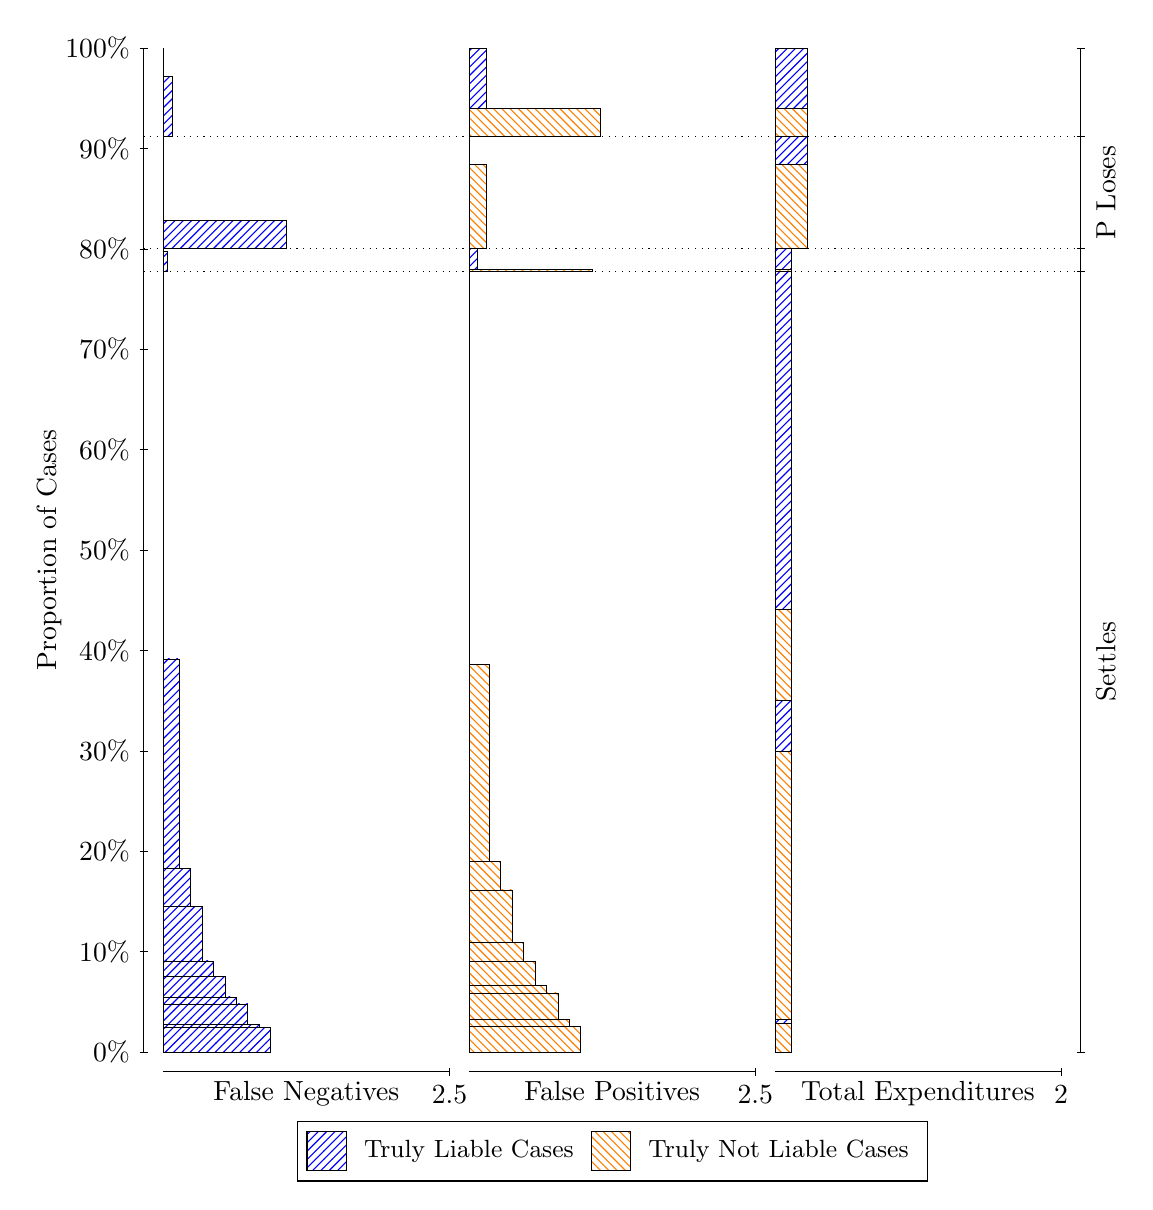
\begin{tikzpicture}
\draw[black, very thin] (1.5,1.75) -- (1.5,14.5);
\node[rotate=90, text=black, anchor=center] at (0.3, 8.125) {Proportion of Cases};
\draw[black, very thin] (1.45,1.75) -- (1.55,1.75);
\node[text=black, anchor=east] at (1.45, 1.75) {0\%};
\draw[black, very thin] (1.45,3.025) -- (1.55,3.025);
\node[text=black, anchor=east] at (1.45, 3.025) {10\%};
\draw[black, very thin] (1.45,4.3) -- (1.55,4.3);
\node[text=black, anchor=east] at (1.45, 4.3) {20\%};
\draw[black, very thin] (1.45,5.575) -- (1.55,5.575);
\node[text=black, anchor=east] at (1.45, 5.575) {30\%};
\draw[black, very thin] (1.45,6.85) -- (1.55,6.85);
\node[text=black, anchor=east] at (1.45, 6.85) {40\%};
\draw[black, very thin] (1.45,8.125) -- (1.55,8.125);
\node[text=black, anchor=east] at (1.45, 8.125) {50\%};
\draw[black, very thin] (1.45,9.4) -- (1.55,9.4);
\node[text=black, anchor=east] at (1.45, 9.4) {60\%};
\draw[black, very thin] (1.45,10.675) -- (1.55,10.675);
\node[text=black, anchor=east] at (1.45, 10.675) {70\%};
\draw[black, very thin] (1.45,11.95) -- (1.55,11.95);
\node[text=black, anchor=east] at (1.45, 11.95) {80\%};
\draw[black, very thin] (1.45,13.225) -- (1.55,13.225);
\node[text=black, anchor=east] at (1.45, 13.225) {90\%};
\draw[black, very thin] (1.45,14.5) -- (1.55,14.5);
\node[text=black, anchor=east] at (1.45, 14.5) {100\%};

\draw[black, very thin] (13.4,1.75) -- (13.4,14.5);
\draw[black, very thin] (13.35,1.75) -- (13.45,1.75);
\node[anchor=west] at (13.35, 1.75) {};
\draw[black, very thin] (13.35,11.661) -- (13.45,11.661);
\node[anchor=west] at (13.35, 11.661) {};
\draw[black, very thin] (13.35,11.953) -- (13.45,11.953);
\node[anchor=west] at (13.35, 11.953) {};
\draw[black, very thin] (13.35,13.378) -- (13.45,13.378);
\node[anchor=west] at (13.35, 13.378) {};
\draw[black, very thin] (13.35,14.5) -- (13.45,14.5);
\node[anchor=west] at (13.35, 14.5) {};

\draw[black, very thin, pattern color=blue, pattern=north east lines] (1.75,1.75) rectangle (3.1125,2.0594);
\draw[black, very thin, pattern color=blue, pattern=north east lines] (1.75,2.0594) rectangle (2.9672,2.1049);
\draw[black, very thin, pattern color=blue, pattern=north east lines] (1.75,2.1049) rectangle (2.8218,2.3595);
\draw[black, very thin, pattern color=blue, pattern=north east lines] (1.75,2.3595) rectangle (2.6765,2.449);
\draw[black, very thin, pattern color=blue, pattern=north east lines] (1.75,2.449) rectangle (2.5312,2.7053);
\draw[black, very thin, pattern color=blue, pattern=north east lines] (1.75,2.7053) rectangle (2.3858,2.9069);
\draw[black, very thin, pattern color=blue, pattern=north east lines] (1.75,2.9069) rectangle (2.2405,3.6024);
\draw[black, very thin, pattern color=blue, pattern=north east lines] (1.75,3.6024) rectangle (2.0952,4.0819);
\draw[black, very thin, pattern color=blue, pattern=north east lines] (1.75,4.0819) rectangle (1.9498,6.7414);
\draw[black, very thin, pattern color=orange, pattern=north west lines] (1.75,6.7414) rectangle (1.75,11.661);
\draw[black, very thin, pattern color=blue, pattern=north east lines] (1.75,11.661) rectangle (1.8045,11.921);
\draw[black, very thin, pattern color=orange, pattern=north west lines] (1.75,11.921) rectangle (1.75,11.953);
\draw[black, very thin, pattern color=blue, pattern=north east lines] (1.75,11.953) rectangle (3.3123,12.314);
\draw[black, very thin, pattern color=orange, pattern=north west lines] (1.75,12.314) rectangle (1.75,13.378);
\draw[black, very thin, pattern color=blue, pattern=north east lines] (1.75,13.378) rectangle (1.859,14.141);
\draw[black, very thin, pattern color=orange, pattern=north west lines] (1.75,14.141) rectangle (1.75,14.5);
\draw[black, very thin, pattern color=orange, pattern=north west lines] (5.6333,1.75) rectangle (7.0503,2.079);
\draw[black, very thin, pattern color=orange, pattern=north west lines] (5.6333,2.079) rectangle (6.905,2.1659);
\draw[black, very thin, pattern color=orange, pattern=north west lines] (5.6333,2.1659) rectangle (6.7597,2.5009);
\draw[black, very thin, pattern color=orange, pattern=north west lines] (5.6333,2.5009) rectangle (6.6143,2.5971);
\draw[black, very thin, pattern color=orange, pattern=north west lines] (5.6333,2.5971) rectangle (6.469,2.902);
\draw[black, very thin, pattern color=orange, pattern=north west lines] (5.6333,2.902) rectangle (6.3237,3.1396);
\draw[black, very thin, pattern color=orange, pattern=north west lines] (5.6333,3.1396) rectangle (6.1783,3.8094);
\draw[black, very thin, pattern color=orange, pattern=north west lines] (5.6333,3.8094) rectangle (6.033,4.1751);
\draw[black, very thin, pattern color=orange, pattern=north west lines] (5.6333,4.1751) rectangle (5.8877,6.6692);
\draw[black, very thin, pattern color=blue, pattern=north east lines] (5.6333,6.6692) rectangle (5.6333,11.661);
\draw[black, very thin, pattern color=orange, pattern=north west lines] (5.6333,11.661) rectangle (7.1957,11.693);
\draw[black, very thin, pattern color=blue, pattern=north east lines] (5.6333,11.693) rectangle (5.7423,11.953);
\draw[black, very thin, pattern color=orange, pattern=north west lines] (5.6333,11.953) rectangle (5.8513,13.018);
\draw[black, very thin, pattern color=blue, pattern=north east lines] (5.6333,13.018) rectangle (5.6333,13.378);
\draw[black, very thin, pattern color=orange, pattern=north west lines] (5.6333,13.378) rectangle (7.3047,13.737);
\draw[black, very thin, pattern color=blue, pattern=north east lines] (5.6333,13.737) rectangle (5.8513,14.5);
\draw[black, very thin, pattern color=orange, pattern=north west lines] (9.5167,1.75) rectangle (9.721,2.1156);
\draw[black, very thin, pattern color=blue, pattern=north east lines] (9.5167,2.1156) rectangle (9.721,2.1612);
\draw[black, very thin, pattern color=orange, pattern=north west lines] (9.5167,2.1612) rectangle (9.721,5.5627);
\draw[black, very thin, pattern color=blue, pattern=north east lines] (9.5167,5.5627) rectangle (9.721,6.2162);
\draw[black, very thin, pattern color=orange, pattern=north west lines] (9.5167,6.2162) rectangle (9.721,7.3682);
\draw[black, very thin, pattern color=blue, pattern=north east lines] (9.5167,7.3682) rectangle (9.721,11.661);
\draw[black, very thin, pattern color=orange, pattern=north west lines] (9.5167,11.661) rectangle (9.721,11.693);
\draw[black, very thin, pattern color=blue, pattern=north east lines] (9.5167,11.693) rectangle (9.721,11.953);
\draw[black, very thin, pattern color=orange, pattern=north west lines] (9.5167,11.953) rectangle (9.9254,13.018);
\draw[black, very thin, pattern color=blue, pattern=north east lines] (9.5167,13.018) rectangle (9.9254,13.378);
\draw[black, very thin, pattern color=orange, pattern=north west lines] (9.5167,13.378) rectangle (9.9254,13.737);
\draw[black, very thin, pattern color=blue, pattern=north east lines] (9.5167,13.737) rectangle (9.9254,14.5);
\draw[black, dotted] (1.5,11.661) -- (13.4,11.661);
\draw[black, dotted] (1.5,11.953) -- (13.4,11.953);
\draw[black, dotted] (1.5,13.378) -- (13.4,13.378);
\draw[black, very thin] (1.75,1.5) -- (5.3833,1.5);
\node[text=black, anchor=north] at (3.5667, 1.5) {False Negatives};
\draw[black, very thin] (5.3833,1.45) -- (5.3833,1.55);
\node[text=black, anchor=north] at (5.3833, 1.45) {2.5};

\draw[black, very thin] (5.6333,1.5) -- (9.2667,1.5);
\node[text=black, anchor=north] at (7.45, 1.5) {False Positives};
\draw[black, very thin] (9.2667,1.45) -- (9.2667,1.55);
\node[text=black, anchor=north] at (9.2667, 1.45) {2.5};

\draw[black, very thin] (9.5167,1.5) -- (13.15,1.5);
\node[text=black, anchor=north] at (11.333, 1.5) {Total Expenditures};
\draw[black, very thin] (13.15,1.45) -- (13.15,1.55);
\node[text=black, anchor=north] at (13.15, 1.45) {2};

\node[text=black, centered, rotate=90] at (13.72, 6.7053) {Settles};

\node[text=black, centered, rotate=90] at (13.72, 12.666) {P Loses};


\draw (7.449999999999999,1.5) node[draw=none] (baseCoordinate) {};
\begin{scope}[align=center]
        \matrix[scale=0.5, draw=black, below=0.5cm of baseCoordinate, nodes={draw}, column sep=0.1cm]{
            \node[rectangle, draw, minimum width=0.5cm, minimum height=0.5cm, pattern color=blue, pattern=north east lines] {}; &
            \node[draw=none, font=\small, text=black] (B) {Truly Liable Cases}; &
            \node[rectangle, draw, minimum width=0.5cm, minimum height=0.5cm, pattern color=orange, pattern=north west lines] {}; &
            \node[draw=none, font=\small, text=black] (B) {Truly Not Liable Cases}; \\
            };
\end{scope}

\end{tikzpicture}
\end{document}